% IEEE conference manuscript. Evidence and build instructions: README.md.
\documentclass[conference]{IEEEtran}
\usepackage{cite}
\usepackage{amsmath,amssymb}
\usepackage{graphicx,booktabs,array}
\usepackage{balance}
\usepackage{xcolor,tikz}
\usetikzlibrary{positioning,arrows.meta}
\usepackage[hidelinks]{hyperref}
\graphicspath{{figures/}}
\newcommand{\model}{MMF-Net}
\newcommand{\bce}{N5\_bce}
\begin{document}
\title{Terrain-Conditioned Deep Neural Networks for\\Next-Day High-Flow Prediction in Sri Lanka}
% Author details remain editable; no identity is inferred.
\author{\IEEEauthorblockN{{[Author Name(s)]}}
\IEEEauthorblockA{\textit{{[Department, Institution]}}\\
{[City]}, Sri Lanka\\{[Email address(es)]}}}
\maketitle

\begin{abstract}
Deep neural networks can combine antecedent rainfall, river discharge and
catchment characteristics for flood-related prediction, but their usefulness
depends on both the representation learned and the validity of the evaluation.
This study examines MMF-Net, a terrain-conditioned temporal transformer for
next-day high-flow prediction at 51 river-basin locations in Sri Lanka. The
network encodes 14-day sequences of 33 dynamic variables using periodic
numerical embeddings, temporal self-attention and cross-feature attention,
with nine static attributes supplied through feature-wise linear modulation.
An optional Sentinel-1 branch supports an exploratory assessment of radar
fusion. The primary target is exceedance of a training-period discharge
percentile in GloFAS-derived data; it is a hydrological proxy rather than an
observed inundation label. In the recorded temporal experiments, replacing
linear embeddings with periodic embeddings increases test average precision
from 0.6083 to 0.7605. The terrain-conditioned five-seed ensemble trained with
binary cross-entropy reaches 0.8355, with a Brier score of 0.0080 and expected
calibration error of 0.0016. These results support further investigation of
numerical representations and static conditioning in neural flood models.
Single-seed ablations, incomplete radar controls and limited agreement between
proxy labels and documented floods constrain interpretation. We identify the
observations and evaluation steps required to assess the model as a
flood-warning decision-support component.
\end{abstract}
\begin{IEEEkeywords}
deep neural networks, temporal transformer, numerical embeddings,
terrain conditioning, flood prediction, Sri Lanka
\end{IEEEkeywords}

\section{Introduction}
Predicting high river flow requires information about both recent weather and
the state of the catchment. Similar rainfall totals can produce different
responses depending on antecedent wetness, existing discharge and local
conditions. A neural forecasting model must therefore represent interactions
among variables as well as their evolution through time. In Sri Lanka, a
dataset spanning contrasting climatic zones provides an opportunity to study
these representations across multiple river-basin locations.

Recurrent neural networks have demonstrated the value of learning
rainfall--runoff relationships from hydrological sequences
\cite{kratzert2018}. More recent large-scale work has extended neural flood
forecasting to ungauged watersheds \cite{nearing2024}. These results motivate
regional studies, but the distinction between the prediction target and the
intended application remains essential. A network trained to reproduce a
discharge reanalysis is evaluated against that reanalysis. Its performance
cannot be interpreted directly as accuracy against measured water levels,
inundation extent or damage.

This paper investigates \model{}, a deep network that combines a temporal
transformer with periodic numerical embeddings, cross-feature attention and
static conditioning. The research emphasis is on neural representation and
fusion: how continuous hydrometeorological inputs are encoded, how static
attributes modify the learned state, and whether an additional radar branch
provides useful information. Conventional reference models provide context
for the difficulty of the target; the principal experiments concern the DNN
and its component ablations.

Three questions guide the analysis: (1) how do numerical embeddings,
cross-feature attention and terrain conditioning affect the recorded neural
prediction scores; (2) how do the training objective and ensemble calibration
affect ranking and probability quality; and (3) what evidence is available for
radar fusion and practical warning use? The contribution is an application
study of established neural components in Sri Lanka, with explicit
experimental controls and limitations.

\section{Related Work}
\subsection{Neural hydrological forecasting}
Following neural rainfall--runoff modelling \cite{kratzert2018}, large-scale
studies have demonstrated prediction of extreme river flows in ungauged
watersheds \cite{nearing2024}. Here the task is daily classification at fixed
Sri Lankan locations using reanalysis supervision, which differs from
operational global forecasting in its scale, target and evaluation.

Local research also motivates neural temporal models. Saubhagya \emph{et al.}
combine a bidirectional LSTM with time-series regression for water-level
forecasting in the Ratnapura area of the Kalu basin \cite{saubhagya2025}.
Differences in target, horizon and data prevent direct comparison with the
present multi-location exceedance task.

\subsection{Representation, conditioning and spatial structure}
Transformers use self-attention to represent relationships among sequence
elements \cite{vaswani2017}. For continuous inputs, Gorishniy \emph{et al.}
show that feature embeddings can improve deep models across several backbones
\cite{gorishniy2022}. We apply their periodic embedding approach before
temporal encoding. Feature-wise linear modulation (FiLM) conditions a learned
representation on auxiliary attributes \cite{perez2018}; here these describe
terrain, climatic zone and network position.

River graphs offer another way to incorporate hydrological structure, although
their benefit must be established against a suitable per-location control.
Kirschstein and Sun found that their neural forecasting models did not benefit
from the supplied river topology \cite{kirschstein2024}. This motivates a
controlled question rather than a presumption that adding edges improves
forecasting. \model{} is graph-free: weights are shared across locations, but
predictions do not exchange messages between them. Earlier graph-network
experiments are discussed separately because their encoder and data extent
differ from those of the main DNN.

\subsection{Probability quality and evaluation}
Focal loss was introduced to address the dominance of easy examples in dense
object detection \cite{lin2017}; its suitability for hydrological
classification is an empirical question. Deep ensembles and temperature
scaling provide established approaches to probability estimation and post-hoc
calibration \cite{lakshminarayanan2017,guo2017}. Under rare positive events,
precision--recall analysis complements threshold-based verification
\cite{saito2015}. Temporally structured observations also require an evaluation
design that respects their dependence \cite{roberts2017}. These ideas inform
our interpretation of the DNN results and their practical limits.

\section{Study Data and Prediction Task}
\label{sec:data}
\subsection{Spatial coverage and input provenance}
The node inventory contains 51 locations in 16 basin or area groups, including
the Colombo metropolitan group. It assigns 31 nodes to the wet zone, 13 to the
dry zone and seven to the intermediate zone. Fig.~\ref{fig:map} shows their
coordinates and the 35 curated directed flow links. These are representative
modelling locations; the experiments do not use measured discharge from 51
gauges. The graph files also contain 204 spatial links for the separate
graph-based models. Lines in the map indicate connectivity and do not trace
surveyed river channels.

\begin{figure}[t]
\centering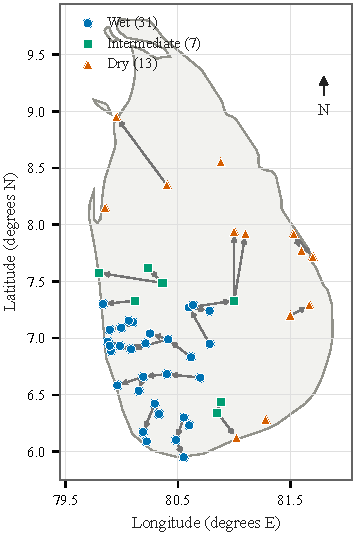
\includegraphics[width=\linewidth]{fig_study_area.pdf}
\caption{Study locations and curated upstream-to-downstream links. Colours and
marker shapes identify the inventory's climatic-zone categories. Country
outline: Natural Earth. Hydrological basin boundaries are not shown.}
\label{fig:map}
\end{figure}

NASA POWER supplies base daily meteorological and soil-wetness variables
\cite{power}. The feature builder preferentially uses cached Open-Meteo
Archive precipitation where available, falling back to POWER precipitation.
The archive request does not pin a particular reanalysis model version.
Discharge is obtained through the Open-Meteo Flood API from the GloFAS product
family \cite{harrigan2020,openmeteo}. Elevation in the supplied node table
comes from POWER response metadata. Product versions and the proportions of
precipitation sources need to be retained in a data manifest to reproduce
the exact historical panel.

The 33 dynamic inputs comprise 11 rainfall and antecedent-rainfall variables,
seven temperature, humidity, wind and radiation variables, six soil-wetness
variables, and nine discharge variables. Discharge features include recent
changes, rolling means, seasonal anomalies and the empirical percentile.
The nine static inputs comprise elevation, log mean-training-discharge as a
drainage proxy, three climatic-zone indicators and four network-position
indicators. The drainage proxy is not a measured catchment area.

Selected heavy-tailed dynamic variables undergo a signed $\log(1+|x|)$
transformation followed by standardisation. Dynamic statistics are fitted on
the temporal training subset. Discharge percentile references and climatologies
are fitted through 2017. Static continuous attributes are standardised across
the node inventory. Missing normalised dynamic values are replaced with zero,
corresponding to the training mean; the main tabular stream has no separate
missingness mask.

\subsection{Targets and episode definition}
Let $Q_{n,t}$ denote reanalysis discharge at location $n$ on day $t$. The
high-flow state and primary next-day target are
\begin{align}
\tau_n &= \operatorname{quantile}_{0.98}
       \{Q_{n,t}:t\leq\text{2017-12-31}\},\\
s_{n,t} &= \mathbf{1}[Q_{n,t}\geq\tau_n],\qquad
y^{(1)}_{n,t}=s_{n,t+1}.
\end{align}
This percentile of daily discharge is a relative high-flow threshold, not a
calibrated return-period estimate or an official warning-stage threshold. It
does not establish whether water leaves the channel or affects settlements.

Auxiliary classification targets indicate any exceedance in the next two and
three days, $y^{(h)}_{n,t}=\max_{k=1,\ldots,h}s_{n,t+k}$, and next-day onset,
$y^{(o)}_{n,t}=(1-s_{n,t})s_{n,t+1}$. Two regression heads predict the next-day
discharge percentile and the maximum discharge z-score over the next three
days. All reported main-model scores concern $y^{(1)}$, not the onset head.

Episodes are constructed separately at each node by grouping positive state
days whose successive dates are at most two days apart. A one-day
non-exceedance gap may therefore lie inside an episode span. These are
node-level proxy episodes: a single storm can produce several episodes at
different nodes. They are not independent national disasters.

\subsection{Coverage and data-version scope}
The main DNN configuration truncates inputs after 31 December 2024. The supplied
episode catalogue contains 1,469 entries through 2025, of which 1,464 start in
2003--2024. Fig.~\ref{fig:episodes} summarises the retained catalogue without
interpreting its annual variation as a trend in observed disasters.

\begin{figure}[t]
\centering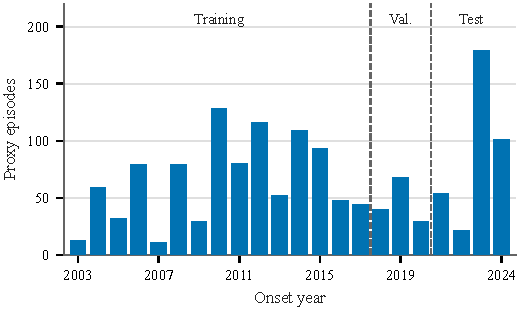
\includegraphics[width=\linewidth]{fig_episode_profile.pdf}
\caption{Annual counts of node-level proxy episodes with onset in 2003--2024,
computed from the supplied catalogue (1,464 entries). Divisions indicate the
temporal training, validation and test periods. These are catalogue counts,
not the episodes eligible for a particular model's evaluation.}
\label{fig:episodes}
\end{figure}

The earlier validation report lists 409,350 valid node-days, including 75,555
test records, but covers a panel extending into 2025. Those totals cannot
describe the truncated DNN experiment without a new panel audit. We report the
protocol dates in Table~\ref{tab:settings} and retain historical performance
values as recorded. Exact post-filter sample counts must be recovered from run
artifacts before submission; the full panel and saved predictions are absent
from the current paper checkout.

\section{Deep Neural Network Method}
\label{sec:method}
\subsection{Numerical and temporal representation}
For a prediction issued after day $t$, the input is
$\mathbf{X}_{n,t}\in\mathbb{R}^{14\times33}$, ending on that day. Nodes are
folded into the batch dimension, so the same network processes every node's
history independently. For scalar feature $j$, the periodic--linear--ReLU
(PLR) representation is
\begin{equation}
\mathbf{e}_j(x)=\operatorname{ReLU}\!\left(
\mathbf{W}_j[\sin(2\pi\mathbf{c}_j x)\Vert
\cos(2\pi\mathbf{c}_j x)]+\mathbf{b}_j\right),
\end{equation}
where $\mathbf{c}_j\in\mathbb{R}^{8}$ contains trainable frequencies and
$\mathbf{e}_j\in\mathbb{R}^{8}$. This supplies a flexible nonlinear
representation before features are mixed; it does not imply that an ordinary
deep network cannot learn nonlinear boundaries.

Each day's feature embeddings are concatenated and projected to a 128-dimensional
token. Learned position embeddings and a classification token are passed through
three pre-layer-normalised transformer blocks, each with four attention heads,
a feed-forward width of 256 and dropout of 0.2. The final classification-token
state is the temporal representation $\mathbf{h}^{T}$.

\subsection{Cross-feature attention and static conditioning}
The feature branch uses the same embeddings, averaged over the 14-day window.
Each feature is projected to a 128-dimensional token with a learned feature
identity. A one-layer transformer pools these tokens to produce
$\mathbf{h}^{F}$. The branches merge additively:
\begin{equation}
\mathbf{h}=\operatorname{LN}(\mathbf{h}^{T}+\mathbf{h}^{F}).
\end{equation}
This branch explicitly attends across feature tokens. Averaging first reduces
its computational cost but removes observation order within each feature token.

An MLP maps the static vector $\mathbf{s}_n\in\mathbb{R}^{9}$ to
$\gamma_n$ and $\beta_n$, giving
\begin{equation}
\widetilde{\mathbf{h}}=\operatorname{LN}
 [\mathbf{h}\odot(1+\gamma_n)+\beta_n].
\end{equation}
The final conditioning layer is zero-initialised, so the initial affine
modulation is neutral. Layer normalisation still applies; the full FiLM block
is not an identity map. A fusion MLP of widths 192 and 128 and a shared head of
widths 256 and 128 produce classification logits and regression outputs.
Fig.~\ref{fig:architecture} shows the implemented data flow.

\begin{figure*}[t]
\centering
\resizebox{\textwidth}{!}{%
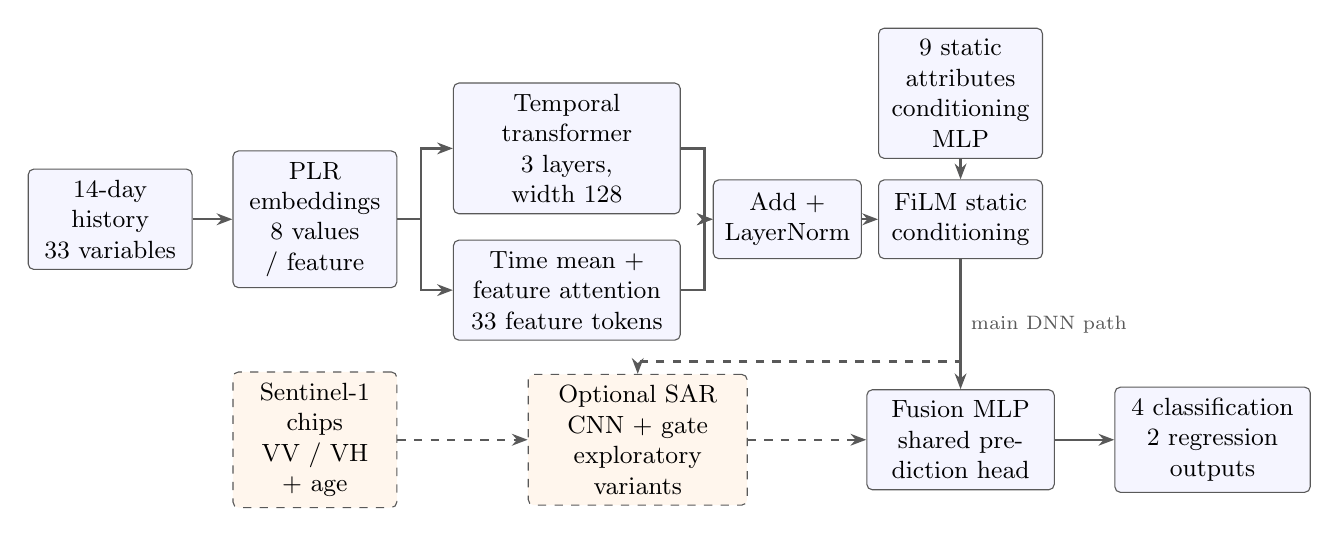
\begin{tikzpicture}[font=\small,
 b/.style={draw=black!65,rounded corners=2pt,align=center,minimum height=10mm,
 text width=1.8cm,inner sep=4pt,fill=blue!4},
 a/.style={-{Stealth[length=2mm]},thick,black!65}]
\node[b] (x) at (0,0) {14-day history\\33 variables};
\node[b] (e) at (2.6,0) {PLR embeddings\\8 values / feature};
\node[b,text width=2.6cm] (t) at (5.8,0.9) {Temporal transformer\\3 layers, width 128};
\node[b,text width=2.6cm] (f) at (5.8,-0.9) {Time mean + feature attention\\33 feature tokens};
\node[b,text width=1.6cm] (m) at (8.6,0) {Add +\\LayerNorm};
\node[b] (film) at (10.8,0) {FiLM static\\conditioning};
\node[b] (s) at (10.8,1.6) {9 static attributes\\conditioning MLP};
\node[b,dashed,fill=orange!7,text width=2.5cm] (sar) at (6.7,-2.8) {Optional SAR CNN + gate\\exploratory variants};
\node[b,dashed,fill=orange!7] (img) at (2.6,-2.8) {Sentinel-1 chips\\VV / VH + age};
\node[b,text width=2.1cm] (head) at (10.8,-2.8) {Fusion MLP\\shared prediction head};
\node[b,text width=2.2cm] (out) at (14,-2.8) {4 classification\\2 regression outputs};
\draw[a] (x)--(e);
\draw[a] (e.east) -- ++(0.3,0) |- (t.west);
\draw[a] (e.east) -- ++(0.3,0) |- (f.west);
\draw[a] (t.east) -- ++(0.3,0) |- (m.west);
\draw[a] (f.east) -- ++(0.3,0) |- (m.west);
\draw[a] (m)--(film); \draw[a] (s)--(film);
\draw[a] (film)--node[right,font=\scriptsize]{main DNN path}(head);
\draw[a,dashed] (film.south) -- ++(0,-1.3) -| (sar.north);
\draw[a,dashed] (img)--(sar);
\draw[a,dashed] (sar)--(head); \draw[a] (head)--(out);
\end{tikzpicture}}
\caption{\model{} data flow. Temporal and cross-feature attention are parallel
branches sharing numerical embeddings. Static attributes condition their
merged state. The principal configuration uses the solid path; optional radar
fusion is applied before the fusion MLP. No graph message passing is used.}
\label{fig:architecture}
\end{figure*}

\subsection{Optional radar branch}
The CNN variant encodes two-channel Sentinel-1 VV/VH chips and adds their
projection through a learned gate. For radar embedding $\mathbf{v}$,
presence indicator $m$ and image age $a$, the fusion is
\begin{align}
\mathbf{g}&=\sigma\{\operatorname{MLP}
 [\widetilde{\mathbf{h}}\Vert\mathbf{v}\Vert m\Vert(a/30)]\},\\
\mathbf{h}^{S}&=\operatorname{LN}
 (\widetilde{\mathbf{h}}+m\,\mathbf{g}\odot\mathbf{W}_v\mathbf{v}).
\end{align}
The gate's final bias is initialised to $-3$, giving a small, nonzero opening;
absent frames contribute zero through $m$. A scalar variant instead appends
four image-derived summaries to the dynamic stream. Experiment notes report
imagery at nine of 51 nodes. Pretraining support exists in the code, but a
completed pretrained checkpoint is not verified in the recorded evidence.
The CNN result is therefore not presented as a validated pretrained-radar
experiment.

\subsection{Multi-task optimisation and calibrated inference}
The reference objective sums masked binary cross-entropy (BCE) over four heads,
with weights $(1.0,0.3,0.3,0.5)$, and adds the mean Huber loss over the two
regressions with weight 0.2. The alternative \texttt{focal\_conf} objective
uses focal loss with $\alpha=0.75$, $\gamma=2$, and a label-confidence weight
between 0.5 and 1 that decreases near the current-day discharge threshold.
The comparison changes class weighting, focusing and confidence weighting
jointly; it is not an isolated test of the focal exponent.

AdamW uses a learning rate of $10^{-3}$, weight decay $10^{-4}$, five warmup
epochs and a cosine schedule. Training lasts at most 60 epochs, with gradient
norm clipping at 1.0 and early-stopping patience of ten. Checkpoints are selected
by validation episode-level average precision, falling back to node-day average
precision if the episode score is undefined.

For five-seed ensembles, the implementation averages predicted probabilities,
not logits. If $p_k$ is the probability from seed $k$, calibration uses
\begin{equation}
\bar p=\frac{1}{5}\sum_{k=1}^{5}p_k,\qquad
p_{\mathrm{cal}}=\sigma\!\left[\frac{\operatorname{logit}(\bar p)}{T}\right].
\end{equation}
The temperature $T$ is fitted on validation data. The decision threshold is
selected by validation F1 and frozen for test evaluation. The reported
operating points do not use a common false-alarm budget.

\section{Experimental Design}
\subsection{Main DNN ablations and historical references}
\begin{table}[t]
\caption{Main temporal DNN configuration.}
\label{tab:settings}
\centering\footnotesize
\begin{tabular}{@{}p{0.42\columnwidth}p{0.52\columnwidth}@{}}
\toprule
Setting & Value \\
\midrule
Training / validation & 2003--2017 / 2018--2020 \\
Test input dates & 2021--2024 \\
Input dimensions & 14 days; 33 dynamic, 9 static \\
Temporal / feature blocks & 3 / 1; width 128, 4 heads \\
Batch size & 32 daily snapshots; CNN: 8 \\
Optimiser / maximum epochs & AdamW / 60 \\
Seeds & N0--N4: 1; N5 and N6: 5 \\
Main target & Next-day discharge exceedance \\
Checkpoint / threshold & Validation episode AP / F1 \\
\bottomrule
\end{tabular}
\end{table}

The main evidence is the August 2026 \model{} result snapshot retained in the
repository. N0--N3 successively introduce PLR embeddings, feature attention and
FiLM conditioning. N4 replaces BCE with \texttt{focal\_conf}; N5 adds a
five-seed ensemble and temperature scaling to that objective. \bce{} applies
the same ensemble procedure to N3 with BCE. N6 variants explore radar scalars
and gated CNN fusion under \texttt{focal\_conf}. The radar rows therefore do
not continue the BCE configuration under a matched objective.

Earlier experiments include a GRU-based spatiotemporal graph network
(TF-STGNN) and persistence, climatology, discharge-percentile and LightGBM
references. Those runs predate the December 2024 truncation policy. A direct
ranking against \model{} would confound data extent with the model. These
historical results appear in a separate table and are excluded from the main
ablation plots.

\subsection{Metrics and their interpretation}
The stored metric named PR-AUC is computed as stepwise average precision (AP),
$\sum_i P_i\Delta R_i$, rather than a trapezoidal area. We use AP throughout.
The implementation sorts individual samples without grouping equal scores;
tied-score references, especially binary persistence, need a standard
tie-aware recomputation before direct comparison.

Node-day quantities are probability of detection,
$\mathrm{POD}=TP/(TP+FN)$; false-alarm ratio,
$\mathrm{FAR}=FP/(TP+FP)$; and critical success index,
$\mathrm{CSI}=TP/(TP+FP+FN)$. FAR is the fraction of positive predictions that
are false alarms, not $FP/(FP+TN)$. Brier score averages $(p-y)^2$.
Expected calibration error (ECE) uses 15 equal-width probability bins,
weighted by sample counts. Under class imbalance, a small aggregate ECE can
coexist with poor calibration in sparsely populated high-risk bins.

Episode detection credits any alarm at a node during the seven days preceding
its episode onset. Validation episode AP scores each eligible episode by the
maximum probability in that window and uses flood-free node-weeks as negatives.
This is a retrospective association statistic. Because the model predicts the
next day, an alarm six days before onset is not evidence of a calibrated six-day
forecast. An onset-specific assessment should align the evaluation window with
the stated horizon and require complete pre-onset coverage.

\section{Results}
\subsection{Neural representation and static conditioning}
Table~\ref{tab:ablation} reports the recorded \model{} results.
PLR embeddings increase AP from 0.6083 to 0.7605, an absolute change of 0.1522.
Feature attention produces a further increase to 0.7738, followed by 0.8269
with static FiLM conditioning. These observations are consistent with the
value of flexible scalar representations and location-dependent conditioning.
The FiLM contrast does not isolate elevation from the drainage proxy, zone and
position indicators supplied to the same module.

\begin{table}[t]
\caption{Main DNN results on the temporal test split.}
\label{tab:ablation}
\centering\footnotesize
\begin{tabular}{@{}llrrrr@{}}
\toprule
ID & Configuration & AP & ECE & FAR & Params \\
\midrule
N0 & Linear embeddings & .6083 & .0024 & .412 & .551 \\
N1 & + PLR & .7605 & .0053 & .325 & .555 \\
N2 & + feature attention & .7738 & .0056 & .313 & .693 \\
N3 & + static FiLM & .8269 & .0032 & .110 & .711 \\
N4 & + focal/confidence & .7592 & .0525 & .138 & .711 \\
N5 & N4, ensemble + TS & .7846 & .0043 & .145 & .711 \\
\bce{} & N3, ensemble + TS & \textbf{.8355} & .0016 & .120 & .711 \\
\midrule
N6-sc & SAR scalars, focal & .7284 & .0055 & .344 & .719 \\
N6-gat & SAR CNN, focal & .8310 & .0066 & .107 & 11.967 \\
\bottomrule
\end{tabular}
\vspace{2pt}
\parbox{\columnwidth}{\scriptsize TS: temperature scaling. N0--N4: one seed;
others: five. Params: millions per member. ``Focal'': combined focal/confidence
objective. Bold marks the largest recorded AP, not significance.
Source: model-2 snapshot, 10--11 August 2026.}
\end{table}

\begin{figure}[t]
\centering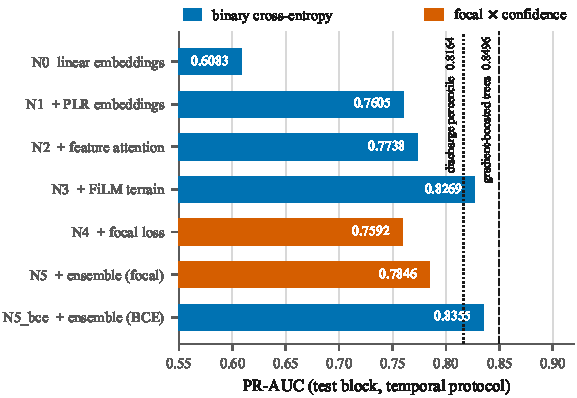
\includegraphics[width=\linewidth]{fig_ladder.pdf}
\caption{Recorded DNN average precision. Points show individual configurations.
Marker shape identifies the training objective. No confidence intervals are
available; the plot does not establish statistical significance.}
\label{fig:ladder}
\end{figure}

N0--N4 each use one seed. Their differences describe these runs rather than
statistically established component effects. The reported 0.3375--0.3856 range
across \bce{} seeds concerns best-validation \emph{episode} AP. It cannot
serve as an uncertainty interval for differences in test \emph{node-day} AP.
Paired test predictions and repeated controlled runs are needed for an
uncertainty analysis on the same estimand.

\subsection{Objective, ensemble and calibration}
Replacing BCE with the combined focal/confidence objective changes N3's AP
from 0.8269 to 0.7592 and ECE from 0.0032 to 0.0525. In the ensemble
comparison, \bce{} records AP 0.8355 and ECE 0.0016, compared with 0.7846 and
0.0043 for N5. These observations favour BCE under the evaluated settings.
They do not establish that focal loss is generally unsuitable for flood
prediction or identify which part of the combined weighting causes the change.

The \bce{} ensemble has reported Brier score 0.0080 and CSI 0.561. Its AP
exceeds N3's by 0.0086. Ensembling and temperature scaling are changed together,
so their separate effects on probability quality are not identified. A positive
temperature preserves score ordering within a fixed ensemble; it changes
probabilities and threshold behaviour rather than AP. Reliability curves, bin
counts and event-stratified calibration would be more informative than ECE
alone, but cannot be recovered from the available aggregate results.

\subsection{Radar fusion and model size}
The scalar radar variant records AP 0.7284. The gated CNN records 0.8310,
compared with 0.7846 for the image-free focal/confidence ensemble and 0.8355
for the image-free BCE ensemble. This is mixed evidence: the CNN result is
higher under the focal/confidence family, yet does not exceed the strongest
recorded image-free result. Differing objectives, batch sizes, uncertain
pretraining status and limited coverage prevent attribution to radar alone.

\begin{figure}[t]
\centering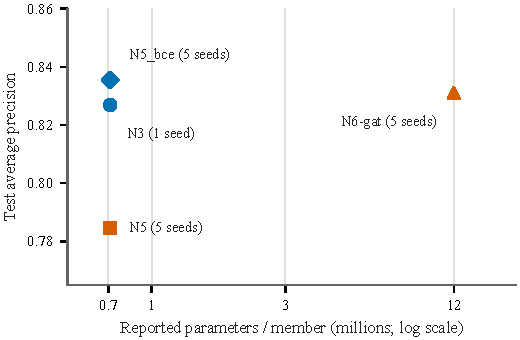
\includegraphics[width=\linewidth]{fig_capacity.pdf}
\caption{Reported parameter count per member and AP for selected DNNs.
The horizontal axis is logarithmic. The gated CNN has about 16.8 times the
reported parameters of the image-free model. Counts do not measure latency,
memory consumption or the benefit of radar information.}
\label{fig:capacity}
\end{figure}

Fig.~\ref{fig:capacity} illustrates the resource implications. \bce{} has
approximately 0.711 million reported parameters per member, whereas N6-gat has
11.967 million. A five-member image-free ensemble stores approximately
3.56 million parameters across its members and requires five forward passes.
The training code counts parameters with gradients enabled, so checkpoint
freeze status must accompany any final model-size comparison. Device-level
latency and deployment energy were not measured.

\subsection{Detection at recorded operating points}
Fig.~\ref{fig:operating} shows event detection alongside node-day FAR for
selected DNN configurations. N2 detects 0.423 of episodes under the seven-day
rule at FAR 0.313; N3 records detection 0.197 at FAR 0.110; and \bce{} records
0.220 at FAR 0.120. Each point reflects both the model and its validation-selected
threshold. These are not points along a shared operating curve and do not
establish which network is preferable at a fixed false-alarm budget.

\begin{figure}[t]
\centering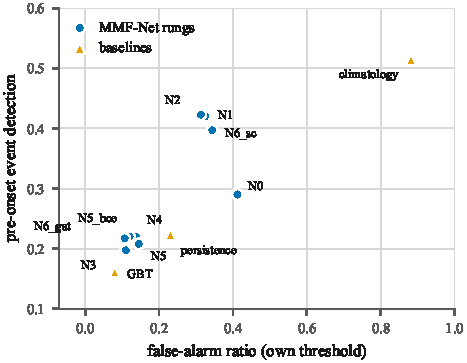
\includegraphics[width=\linewidth]{fig_operating_points.pdf}
\caption{Selected DNN operating points. Detection credits any alarm in the
seven days before onset; FAR is calculated over node-days. Each point uses
its own validation-selected threshold. The axes have different aggregation
units and are not an event-level precision--recall curve.}
\label{fig:operating}
\end{figure}

\subsection{Historical references and split diagnostics}
\begin{table}[t]
\caption{Historical references (2 August 2026); panel extent differs from
Table~\ref{tab:ablation}. Dashes indicate unavailable values.}
\label{tab:legacy}
\centering\footnotesize
\begin{tabular}{@{}lrrrr@{}}
\toprule
Reference & AP & Brier & FAR & Detection \\
\midrule
Persistence & .590 & -- & .231 & .223 \\
Climatology & .108 & -- & .882 & .515 \\
Discharge percentile & .816 & -- & .231 & .223 \\
LightGBM & .8496 & .0076 & .080 & .161 \\
GRU only (M0) & .598 & .0137 & .441 & .262 \\
TF-STGNN (M3) & .704 & .0135 & .342 & .380 \\
\bottomrule
\end{tabular}
\end{table}

The historical discharge-percentile reference achieves AP approximately 0.816,
consistent with substantial persistence in a next-day discharge target.
LightGBM records 0.8496 on its historical panel (Table~\ref{tab:legacy}).
These values motivate strong references in a matched rerun; they do not
establish a DNN-versus-tree ordering on an identical test set. Comparing
graph-based M3 with \model{} would likewise change the encoder and panel as
well as graph structure.

The M3 diagnostic records AP 0.704 under temporal splitting and 0.905 under
random splitting, while seven-day event detection changes from 0.380 to 0.089.
The random protocol interleaves node-days across train and test. Furthermore,
the event routine receives only held-out rows: random masking can remove
pre-onset alarm opportunities and shift the first observed episode day. The
diagnostic demonstrates sensitivity to the split, but does not isolate a causal
loss of warning skill or prove memorisation of neighbouring days. The Gin
holdout (AP 0.840) concerns spatial transfer on four inventory nodes, with
training at other nodes spanning later dates. It is not a future-time test.
Strict spatial evaluation also requires reconsidering held-out-node
preprocessing statistics and graph access.

\section{Practical Interpretation and Limitations}
\subsection{From proxy prediction to warning support}
The proposed use is a candidate ranking and probability component for an
analyst's river-monitoring workflow. A practical workflow would assemble
available inputs at a defined daily issue time, verify freshness and coverage,
run the network, and present probabilities alongside measured water levels and
recent rainfall. The responsible agency would determine how outputs relate to
local warning stages and actions. This is a proposed application, not a system
validated by the present experiments.

The one-day target requires particular care. A daily total for day $t$ is fully
known only after that day, and reanalysis fields may be published or revised
later. Operational lead time must be measured from actual input availability,
not simply from date labels. Replay using archived, issue-time observations
and forecasts is needed before claiming 24-hour warning capability. Radar
images must similarly be restricted to acquisitions available at issue time,
with image age tracked explicitly.

\subsection{Independent evidence and failure cases}
The historical validation report compares the proxy state against selected
documented flood windows. Restricting its list to 2003--2024, the high-flow
threshold activates in seven of ten windows; the lower threshold activates in
eight. The high threshold misses the listed May 2003, June 2014 and May 2017
windows. This is a limited check of label agreement, not DNN event detection,
and it does not estimate warning accuracy on a representative sample. The
reported successes also use basin-level matching and expanded date windows,
which are less demanding than correct daily predictions at individual nodes.

Observed gauge levels, discharge and independently mapped inundation would
allow evaluation of failures that reanalysis labels cannot expose. Cases
should include missed floods, false alarms, rapid-onset events and regulated
rivers, alongside correct predictions. An event hydrograph should display
issue time, available rainfall and discharge, model probability, the frozen
threshold and independently recorded onset. Such plots require aligned
observations and predictions; aggregate scores cannot supply them.

\balance
\subsection{Temporal boundaries and reproducibility}
The 14-day windows may include earlier-period features at split boundaries.
Using preceding validation-period observations to initialise a test forecast
is causal when those observations were available. A separate issue arises
because auxiliary future targets are constructed before split assignment and
input truncation. Horizons near a boundary can reach into the next block or
beyond the declared input end date. A final rerun should purge boundary-crossing
supervised targets and verify complete horizons explicitly.

Scores were retained from a hand-compiled experiment snapshot; underlying
predictions, exact run manifests and post-truncation counts must accompany a
submission. Repeated inspection of the same test set during architecture
development also means these results should be treated as development evidence.
A new time period or prespecified external evaluation is needed for final
confirmation.

\subsection{Priority experiments}
The next DNN comparison should hold the panel, targets, seeds, optimisation
budget and test rows fixed. It should repeat the embedding and FiLM ablations,
separating static-attribute contributions where possible. Graph message passing
can then be added to the same encoder; the unrun STG-Former implementation in
the repository is not evidence of a benefit. A radar comparison should use the
same BCE objective, a documented checkpoint, and results on both common-coverage
nodes and the complete panel.

For decision-oriented evaluation, thresholds should be fitted on validation
under a stated FAR constraint and then frozen. Realised test FAR must still
be reported because the validation constraint may not hold under distribution
shift. Event detection should require full pre-onset coverage and horizon-aligned
alarms, supplemented by false warning episodes per basin-month. Paired
uncertainty intervals should preserve storm or temporal dependence across
nodes; calibration should include bin counts and high-probability subsets.
These are additional experiments, not outcomes of the current study.

\section{Conclusion}
This study examines a terrain-conditioned deep neural network for next-day
high-flow prediction at Sri Lankan river-basin locations. Recorded ablations
show improvements after periodic numerical embeddings and static FiLM
conditioning are introduced, while the BCE ensemble attains the highest
recorded \model{} AP of 0.8355. Radar results remain exploratory and the
available experiments do not isolate the value of graph structure. The findings
support further controlled study of neural representation and fusion.
Establishing a practical warning benefit requires independent flood observations,
issue-time input replay and matched evaluation of onset detection, false alarms
and probability calibration.

\section*{Data and Code Availability}
Code and catalogue files are available at
\url{https://github.com/heshannethmina/Srilanka-Flood-Data-Set-Creation}.
The complete training panel, checkpoints and predictions are absent from the
reviewed checkout. Figure inputs and provenance accompany the manuscript.

\section*{Acknowledgment}
We acknowledge NASA POWER, Copernicus GloFAS, Open-Meteo and Sentinel-1 data
providers, public flood-report sources and Natural Earth.

\begin{thebibliography}{00}
\bibitem{kratzert2018} F. Kratzert, D. Klotz, C. Brenner, K. Schulz, and
M. Herrnegger, ``Rainfall--runoff modelling using Long Short-Term Memory (LSTM)
networks,'' \emph{Hydrol. Earth Syst. Sci.}, vol. 22, pp. 6005--6022, 2018,
doi: 10.5194/hess-22-6005-2018.
\bibitem{nearing2024} G. Nearing \emph{et al.}, ``Global prediction of extreme
floods in ungauged watersheds,'' \emph{Nature}, vol. 627, pp. 559--563, 2024,
doi: 10.1038/s41586-024-07145-1.
\bibitem{saubhagya2025} S. Saubhagya, C. Tilakaratne, P. Lakraj, and
M. Mammadov, ``A fusion of deep learning and time series regression for flood
forecasting: An application to the Ratnapura area based on the Kalu river basin
in Sri Lanka,'' \emph{Forecasting}, vol. 7, no. 2, art. 29, 2025,
doi: 10.3390/forecast7020029.
\bibitem{vaswani2017} A. Vaswani \emph{et al.}, ``Attention is all you need,''
in \emph{Advances in Neural Information Processing Systems}, vol. 30, 2017.
\bibitem{gorishniy2022} Y. Gorishniy, I. Rubachev, and A. Babenko, ``On
embeddings for numerical features in tabular deep learning,'' in
\emph{Advances in Neural Information Processing Systems}, vol. 35, 2022.
\bibitem{perez2018} E. Perez, F. Strub, H. de Vries, V. Dumoulin, and
A. Courville, ``FiLM: Visual reasoning with a general conditioning layer,''
in \emph{Proc. AAAI}, vol. 32, no. 1, 2018,
doi: 10.1609/aaai.v32i1.11671.
\bibitem{kirschstein2024} N. Kirschstein and Y. Sun, ``The merit of river
network topology for neural flood forecasting,'' in \emph{Proc. ICML},
PMLR vol. 235, pp. 24713--24725, 2024.
\bibitem{lin2017} T.-Y. Lin, P. Goyal, R. Girshick, K. He, and P. Doll\'{a}r,
``Focal loss for dense object detection,'' in \emph{Proc. ICCV},
pp. 2980--2988, 2017.
\bibitem{lakshminarayanan2017} B. Lakshminarayanan, A. Pritzel, and C. Blundell,
``Simple and scalable predictive uncertainty estimation using deep ensembles,''
in \emph{Advances in Neural Information Processing Systems}, vol. 30, 2017.
\bibitem{guo2017} C. Guo, G. Pleiss, Y. Sun, and K. Q. Weinberger,
``On calibration of modern neural networks,'' in \emph{Proc. ICML},
PMLR vol. 70, pp. 1321--1330, 2017.
\bibitem{saito2015} T. Saito and M. Rehmsmeier, ``The precision-recall plot is
more informative than the ROC plot when evaluating binary classifiers on
imbalanced datasets,'' \emph{PLOS ONE}, vol. 10, no. 3, art. e0118432, 2015,
doi: 10.1371/journal.pone.0118432.
\bibitem{roberts2017} D. R. Roberts \emph{et al.}, ``Cross-validation strategies
for data with temporal, spatial, hierarchical, or phylogenetic structure,''
\emph{Ecography}, vol. 40, no. 8, pp. 913--929, 2017,
doi: 10.1111/ecog.02881.
\bibitem{power} NASA POWER, ``Meteorology: Data sources and methodology.''
[Online]. Available: \url{https://power.larc.nasa.gov/docs/methodology/meteorology/}.
Accessed: Sep. 8, 2026.
\bibitem{harrigan2020} S. Harrigan \emph{et al.}, ``GloFAS-ERA5 operational
global river discharge reanalysis 1979--present,'' \emph{Earth Syst. Sci. Data},
vol. 12, pp. 2043--2060, 2020, doi: 10.5194/essd-12-2043-2020.
\bibitem{openmeteo} Open-Meteo, ``Flood API.'' [Online]. Available:
\url{https://open-meteo.com/en/docs/flood-api}. Accessed: Sep. 8, 2026.
\end{thebibliography}
\end{document}
